% Midterm Progress Update LaTeX (Fall 2025 598)
% Based on: Certificated Actor-Critic: Hierarchical Reinforcement Learning with Control Barrier Functions for Safe Navigation (central reference).
% Section layout and headings adapted from Prof. Si's 598 report template.
\documentclass[10pt,conference]{IEEEtran}

\usepackage[utf8]{inputenc}
\usepackage[T1]{fontenc}
\usepackage{amsmath,amssymb,amsfonts}
\usepackage{bm}
\usepackage{graphicx}
\usepackage{booktabs}
\usepackage{algorithm}
\usepackage{algpseudocode}
\usepackage{hyperref}
\usepackage{xcolor} % Added to support the \todo command
\hypersetup{hidelinks}

\newcommand{\todo}[1]{\textcolor{red}{[TODO: #1]}}
\newcommand{\etal}{\textit{et al.}}

\begin{document}

\title{Midterm Progress Update:\\
Safe Robot Navigation with Certificated Actor--Critic (CAC)\\
\large A Hierarchical Reinforcement Learning Approach with Control Barrier Functions}

\author{
\IEEEauthorblockN{Team 01: Jeevan Hebbal Manjunath, Varun Karthik, Yeshwanth Reddy Gurureddy}
\IEEEauthorblockA{\quad Emails: \{jhebbalm@asu.edu, vnolas82@asu.edu, ygurredd@asu.edu\}}
}

\maketitle

\begin{abstract}
Our focus is to study safe autonomous navigation using the Certificated Actor--Critic (CAC) framework, a hierarchical reinforcement learning approach that uses Control Barrier Functions (CBFs) to enforce safety constraints. Unlike existing methods that can be myopic or computationally intensive, CAC operates in two stages. First, a \emph{safety critic} is constructed using a CBF-derived reward, yielding a quantitative safety certificate. Second, a task objective like goal-reaching is optimized via a \emph{restricted policy update} that preserves the learned safety guarantees.

Our progress focuses on evaluating this framework on mobile robot and AUV navigation tasks. The reference paper validates this approach with results showing high success and low collision rates, significantly outperforming baseline models with simple reward trade-offs or unrestricted updates. These experiments confirm the safety critic is a reliable indicator of navigation safety, establishing CAC as a practical approach for developing RL policies with measurable, certificate-guided guarantees.
\end{abstract}



\begin{IEEEkeywords}
Safe reinforcement learning, control barrier functions, hierarchical RL, navigation, autonomous robots
\end{IEEEkeywords}

\section{Introduction}

Ensuring \emph{safety} during navigation is a prerequisite for deploying robots in proximity to people and assets. While reinforcement learning (RL) is attractive for its ability to adapt to complex dynamics and partial knowledge, standard RL methods offer weak guarantees under distribution shift or during exploration. \emph{Control Barrier Functions} (CBFs) provide a principled route to enforce the forward invariance of a safe set, yet many CBF-based controllers are either myopic (e.g., pointwise quadratic programs) or rely on simplified models that do not transfer well to complex, real-world environments.

Our project analyzes the \textbf{Certificated Actor--Critic (CAC)} framework \cite{Xie2025CAC}, which proposes a two-stage hierarchical RL design. First, it learns a \emph{safety critic} using a CBF-derived reward; second, it performs a \emph{restricted policy update} that improves task performance while provably not degrading safety as measured by the critic. The CAC method has demonstrated competitive results on the CartPole balancing task and in dense-obstacle \emph{underwater vehicle} navigation. We selected CAC as our central reference for three key reasons: (1) it isolates safety from task optimization through staged training; (2) it endows the critic with the formal meaning of a \emph{quantitative safety certificate}; and (3) it introduces a practical restricted-gradient update that enforces a “do-no-harm” approach to safety during policy improvement.

This research direction is particularly timely, as evidenced by complementary recent work. Studies from 2024--2025 have surveyed the learning of CBFs and their application in safe RL \cite{Guerrier2024Survey}, explored barrier-inspired reward shaping \cite{Ranjan2024BarrierShaping}, and deployed learned neural CBFs on physical robots for navigation \cite{Harms2024NeuralCBF}.

\textbf{Scope.} The application under study is \emph{navigation with formal safety guarantees}, a critical capability for mobile robots, AUVs/ROVs, UGVs, and aerial robots operating in cluttered and uncertain environments.

\textbf{Progress Update.} This report documents our progress by: (i) formalizing the safe navigation problem; (ii) analyzing the core algorithmic choices within the CAC framework; (iii) initiating a replication of the baseline from the reference paper; (iv) presenting preliminary findings from our initial experiments; and (v) outlining a revised evaluation plan to guide future work.

\section{Problem Context and Formulation}

\textbf{Task Definition.} Given a robot governed by discrete-time dynamics $s_{t+1}=F(s_t,a_t)$, with state $s_t\in\mathcal{S}$ and action $a_t\in\mathcal{A}$, the objective is to learn a policy that both (i) remains within a predefined \emph{safe set} $\mathcal{C}=\{s: h(s)\ge 0\}$ and (ii) reaches a navigation goal efficiently.\footnote{We adopt the standard CBF definitions for a safe set and forward invariance as detailed in the central reference paper \cite{Xie2025CAC}.} The discrete-time CBF, $h(\cdot)$, enforces the forward invariance condition via a decay parameter $\alpha\in(0,1)$. The project’s specific \emph{navigation application} is to reach a target location in a cluttered map without collisions, under conditions of noisy sensing and approximate dynamics.

\textbf{Problem Statement.}
This work aims to learn a policy $\pi_\theta$ that satisfies three primary objectives:
\begin{itemize}
    \item \textbf{Safety Guarantee}: Ensure that the state remains within the safe set, $s_t\in \mathcal{C}$, for all timesteps $t$ (forward invariance).
    \item \textbf{Goal Reaching}: Reach the target goal $g$ with near-minimal time or path cost.
    \item \textbf{Quantified Safety}: Provide a numeric, verifiable certificate of safety for any given policy and state.
\end{itemize}
This report adopts the CAC method as the foundational approach. Our analysis focuses on assessing how effectively its \emph{safety critic} provides actionable, quantitative signals for guiding policy updates toward verifiably safe and effective navigation.

\section{Methodology: The Certificated Actor-Critic Framework}
\subsection{Two-Stage Hierarchical RL}
The CAC algorithm decomposes the navigation problem into two stages: \emph{Stage~1: Safety Critic Construction} and \emph{Stage~2: Restricted Policy Update}, as illustrated in Fig.~\ref{fig:framework}.\footnote{Algorithm~1 and Fig.\,1 appear on p.\,2 of \cite{Xie2025CAC}.} In Stage~1, the reward is derived from the CBF invariance condition to learn a safe policy. In Stage~2, a goal-reaching reward is introduced, and policy updates are constrained to ensure the safety value does not degrade \cite{Xie2025CAC}.

\begin{figure}[t]
    \centering
    % NOTE: You will need to provide the 'framework.png' image file.
    % The 'draft' option in \documentclass will show a placeholder box.
    % Remove 'draft' once the image is available.
    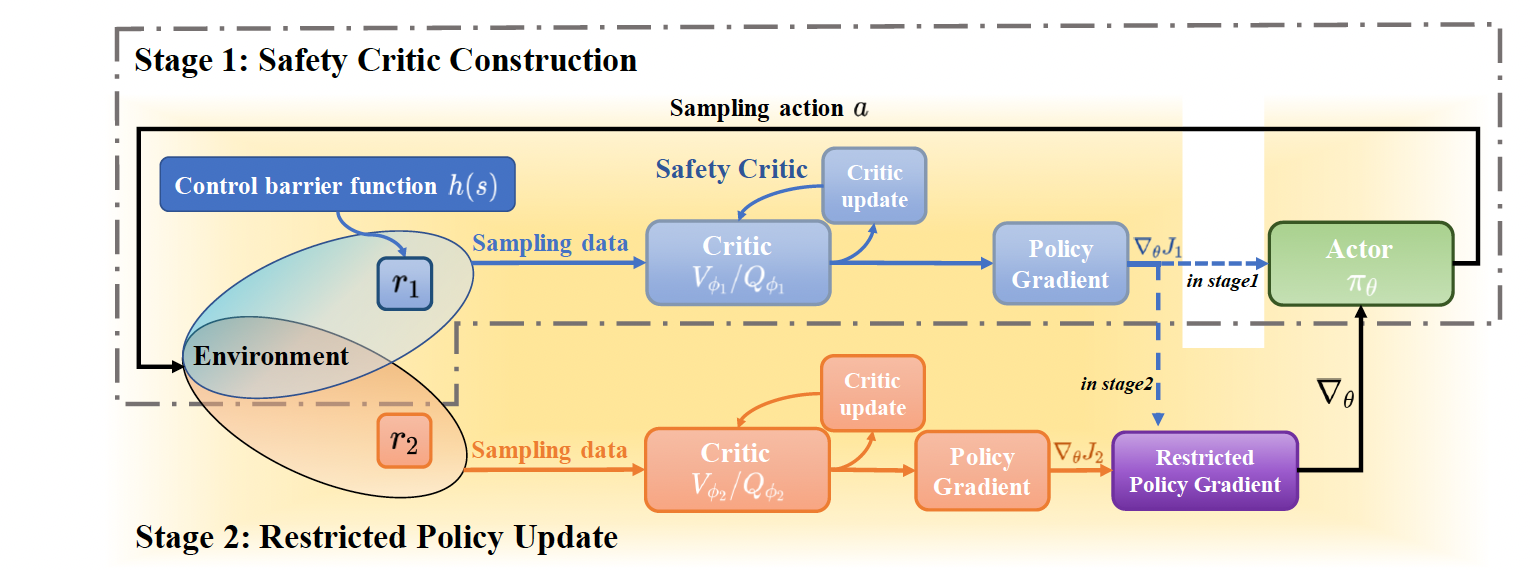
\includegraphics[width=\columnwidth]{CAC_framework.png} 
    \caption{Conceptual diagram of the two-stage Certificated Actor-Critic (CAC) algorithm, adapted from \cite{Xie2025CAC}. Stage 1 trains a safety critic ($Q_1$) using a CBF-based reward ($r_1$). Stage 2 trains a task critic ($Q_2$) on a task reward ($r_2$), using a restricted gradient to update the actor without compromising the safety guarantees learned in Stage 1.}
    \label{fig:framework}
\end{figure}

\subsection{Safety Critic via CBF-Derived Reward}
Let $h(\cdot)$ be a CBF with expected decay $\alpha_0\in(0,1)$. The per-step safety reward is defined as
\begin{equation}
r_1(s_t,a_t)=\exp\Big(\min\big(h(s_{t+1})+(\alpha_0-1)h(s_t),\,0\big)\Big)\in(0,1],
\label{eq:cbf-reward}
\end{equation}
where $s_{t+1}=F(s_t,a_t)$. Training an actor--critic on $r_1$ yields value functions $(V_1,Q_1)$ that serve as \emph{safety critics}: if $V_1(s_0)$ (or $Q_1(s_0,a_0)$) attains its maximal value, the episode is guaranteed to be safe from that state (or state-action pair).\footnote{The safety-certificate interpretation follows Theorem~1 and Eqs.\,(7),(12); see pp.\,2–4 of \cite{Xie2025CAC}.}

\subsection{Goal-Reaching and Restricted Policy Update}
For the goal-reaching task, a control Lyapunov function (CLF) $l(\cdot)$ can be used to define the reward:
\begin{equation}
r_2(s_t,a_t)=-\max\big(l(s_{t+1})+(\beta_0-1)l(s_t),\,0\big),
\label{eq:clf-reward}
\end{equation}
with decay $\beta_0\in(0,1)$. To avoid degrading safety when improving $J_2$ (the actor’s objective under $r_2$), CAC computes a \emph{restricted} policy-gradient direction $e$ that maximizes improvement on $J_2$ while maintaining a non-negative correlation with the safety objective $J_1$:
\begin{align}
\max_{e} \quad & e\cdot\nabla_\theta J_2(\theta) \nonumber\\
\text{s.t.}\quad & e\cdot\nabla_\theta J_1(\theta)\ge 0, \quad \|e\| \le \|\nabla_\theta J_2(\theta)\|.
\label{eq:restricted}
\end{align}
This implements a first-order \emph{do-no-harm} constraint on safety during policy improvement (Eq.\,(10), p.\,4 of \cite{Xie2025CAC}).

\begin{algorithm}[t]
\caption{High-level sketch of the two-stage CAC algorithm, adapted from \cite{Xie2025CAC}}
\begin{algorithmic}[1]
\State \textbf{Input:} CBF $h(\cdot)$ with decay $\alpha_0$; CLF $l(\cdot)$ with decay $\beta_0$
\State \textbf{Stage 1 (Safety critic).} Train actor/critic on $r_1$ in \eqref{eq:cbf-reward} to obtain a safe policy $\pi_{\text{safe}}$ and safety critics $V_1, Q_1$.
\State \textbf{Stage 2 (Restricted update).} Train on $r_2$ in \eqref{eq:clf-reward} using the restricted gradient \eqref{eq:restricted} to improve task performance while preserving safety.
\State \textbf{Output:} Final policy $\pi^\star$ and safety critics $V_1, Q_1$.
\end{algorithmic}
\end{algorithm}

\subsection{Planned Implementation}
We will implement and evaluate the CAC framework on two navigation benchmarks:
\begin{itemize}
    \item \textbf{2D Mobile Robot:} A simulated robot in a continuous 2D plane with circular obstacles, using range-finder-like observations.
    \item \textbf{AUV Navigation:} A 2D simulation mirroring the paper’s HoloOcean setup, with 9-beam range sensing, randomized cubic obstacles, and random start/goal locations to allow for direct comparison.
\end{itemize}
Our implementation includes comprehensive logging to analyze: (i) heatmaps of safety critic values, (ii) safe-episode and success rates, (iii) navigation return, and (iv) training curves comparing CAC with and without the restricted gradient.

\section{Preliminary Results}
Our midterm progress includes the implementation of a 2D navigation environment and a series of baseline experiments. These experiments validate our implementation and clearly motivate the hierarchical approach of the CAC framework.

\begin{figure}[h!]
    \centering
    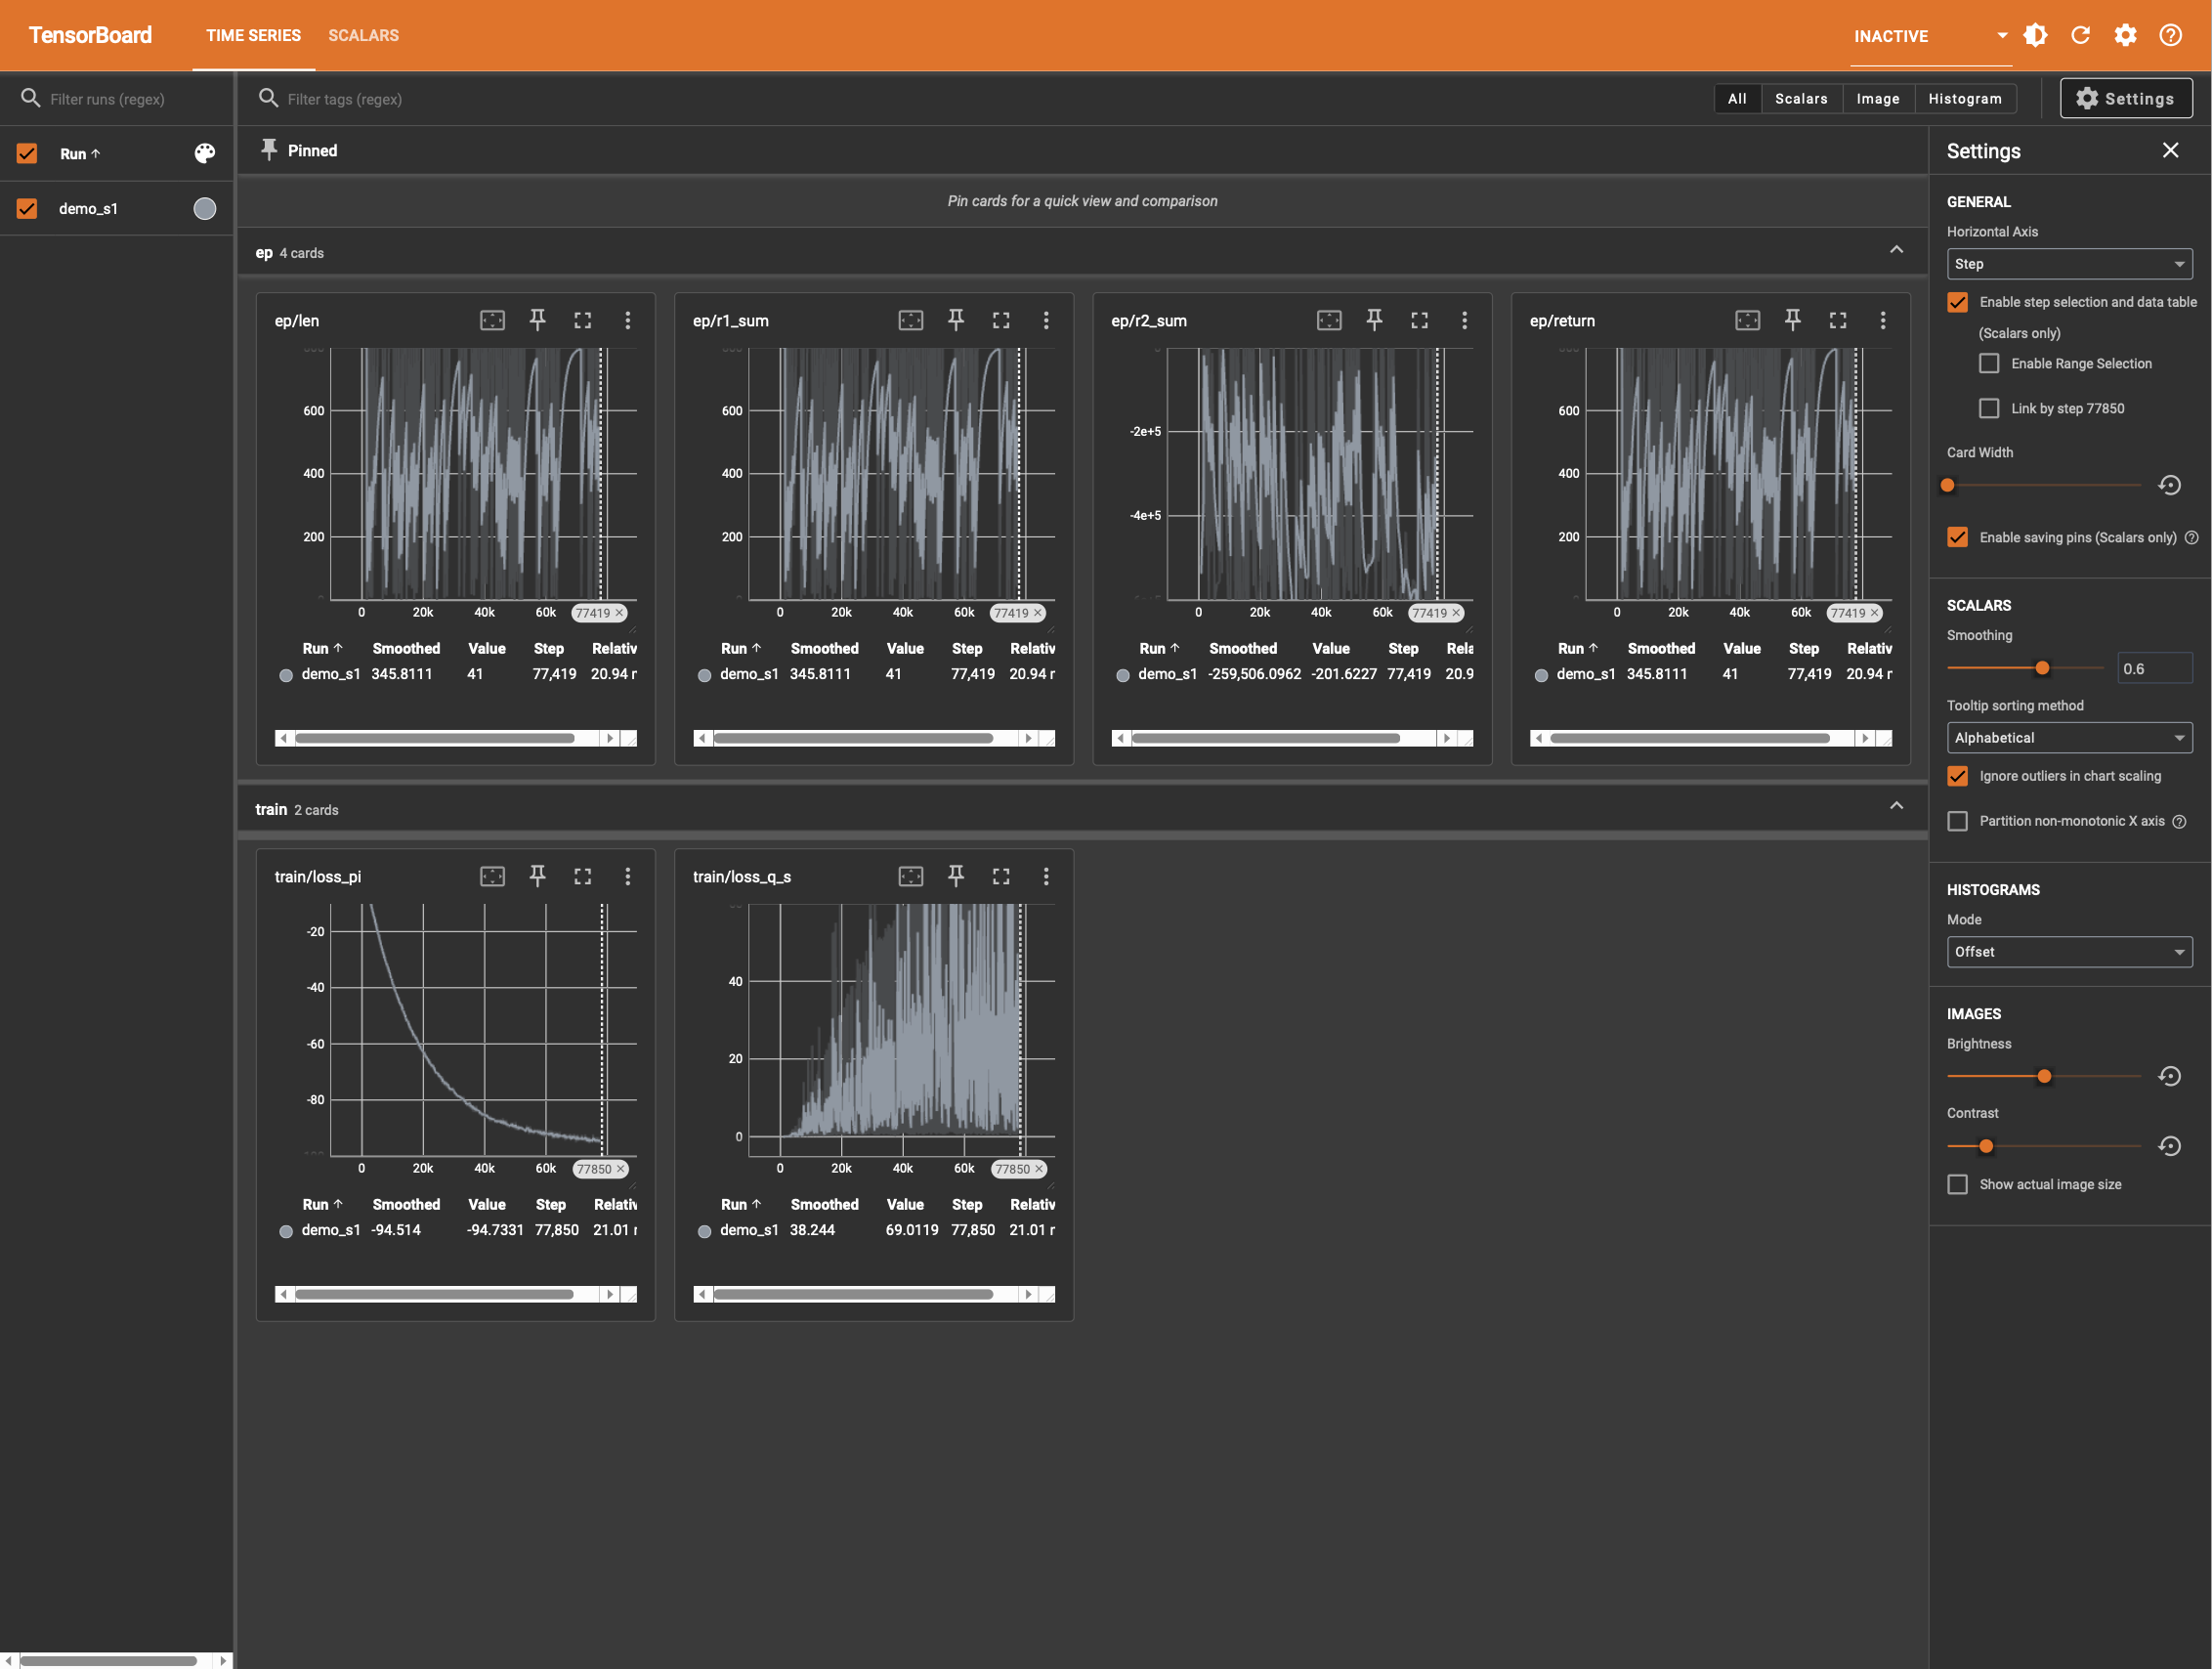
\includegraphics[width=\columnwidth]{tensor_board_for_safety_policy.png}
    \caption{TensorBoard logs from the Stage 1 (Safety-Only) training run. The convergence of actor and critic losses (bottom row) and the stabilization of episode returns and lengths (top row) indicate a successful and stable learning process.}
    \label{fig:safety_training}
\end{figure}

\begin{figure}[h!]
    \centering
    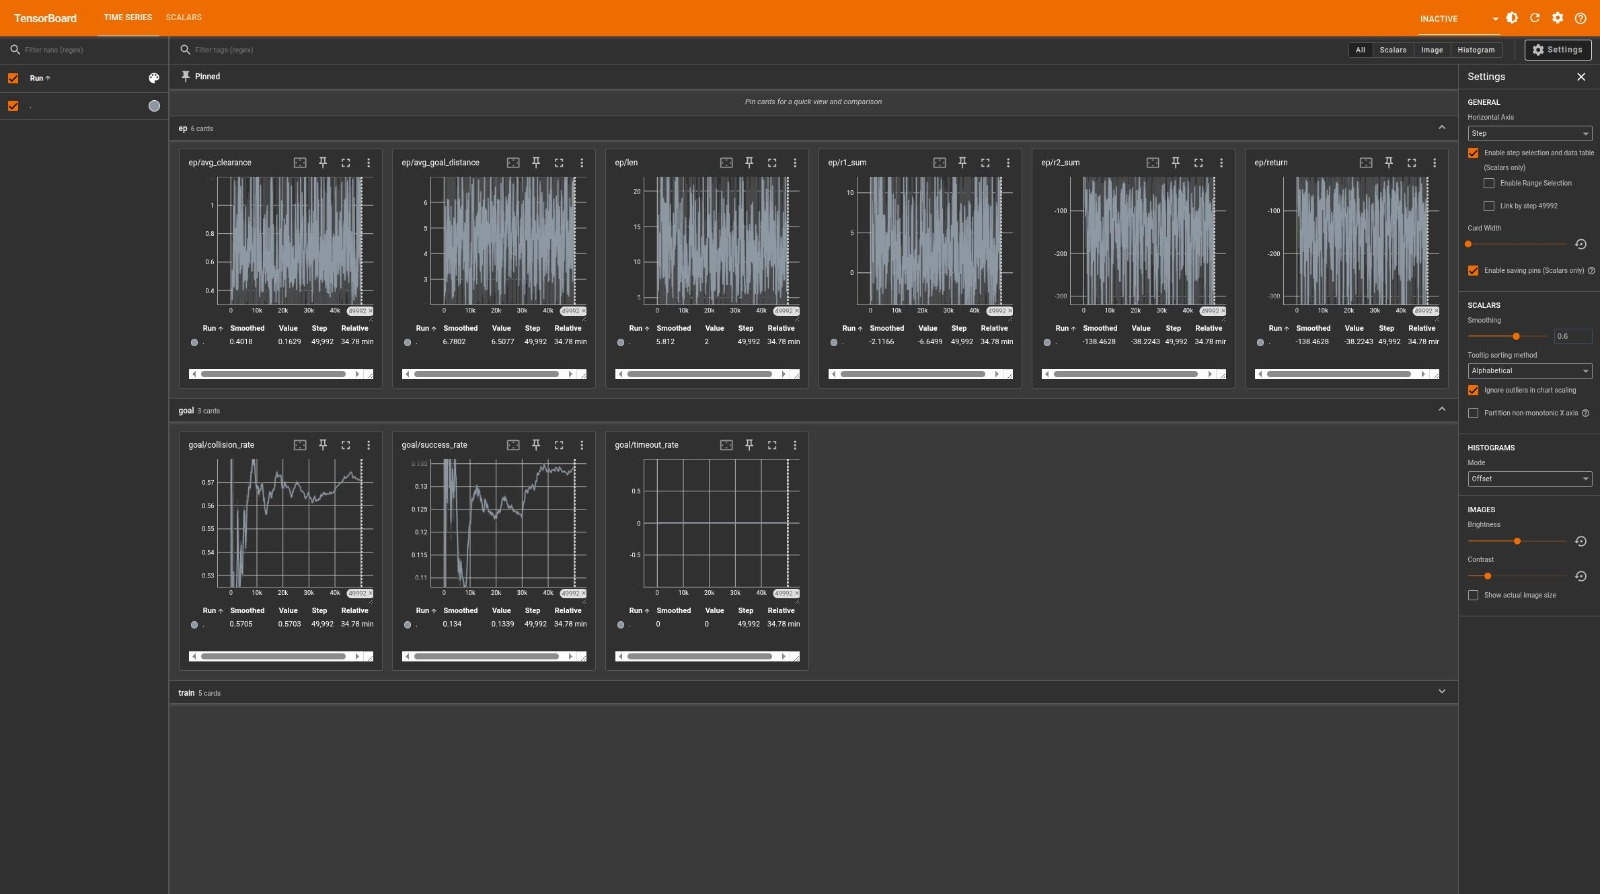
\includegraphics[width=\columnwidth]{model_training.jpeg}
    \caption{TensorBoard logs from the Goal-Only baseline training run. Metrics such as goal distance converge, while the goal collision rate remains high, indicating the agent is learning to reach the goal but without regard for safety.}
    \label{fig:goal_training}
\end{figure}

\begin{figure}[h!]
    \centering
    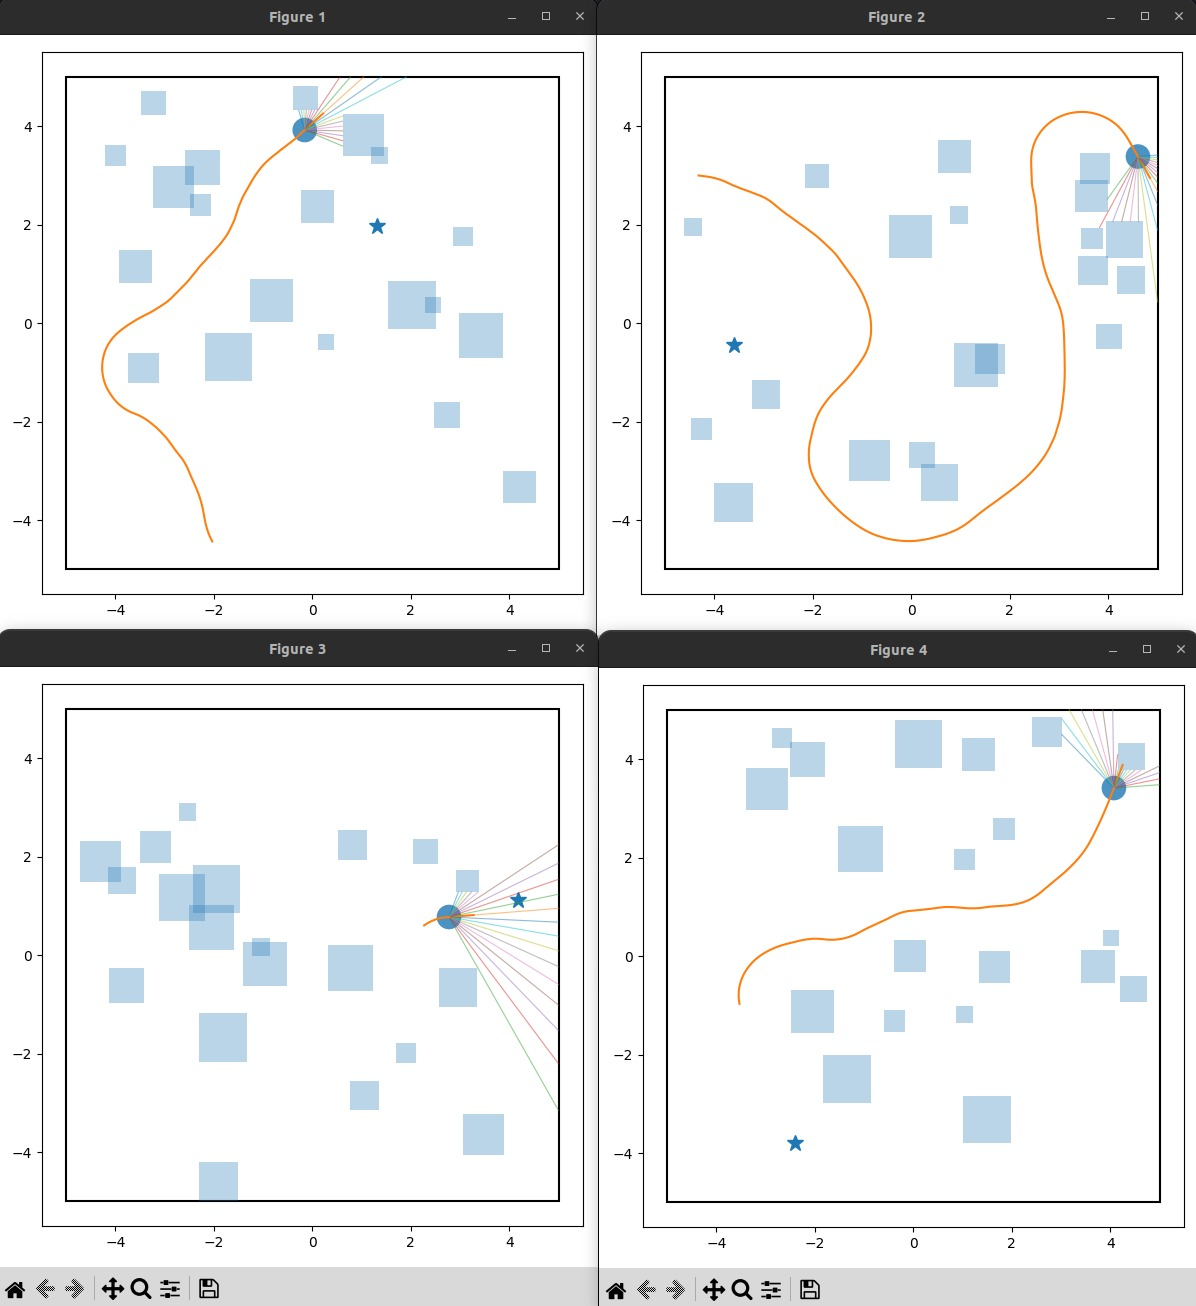
\includegraphics[width=\columnwidth]{safety_only.png}
    \caption{Qualitative results from our implemented Stage 1 (safety-only) policy. The agent successfully generates smooth, collision-free trajectories toward a goal (blue star) in environments with randomly placed obstacles.}
    \label{fig:safety_only}
\end{figure}

\begin{table}[h!]
\caption{Performance Comparison of Baseline Models}
\label{tab:baseline_comparison}
\centering
\begin{tabular}{@{}lccc@{}}
\toprule
Metric & Safety-Only & Goal-Only & Balanced \\ \midrule
Success Rate & 50.0\% & 30.0\% & 36.7\% \\
Collision Rate & \textbf{30.0\%} & 70.0\% & 63.3\% \\
Avg. Clearance (m) & 1.029 & 0.869 & N/A \\ \bottomrule
\end{tabular}
\end{table}

\begin{figure}[h!]
    \centering
    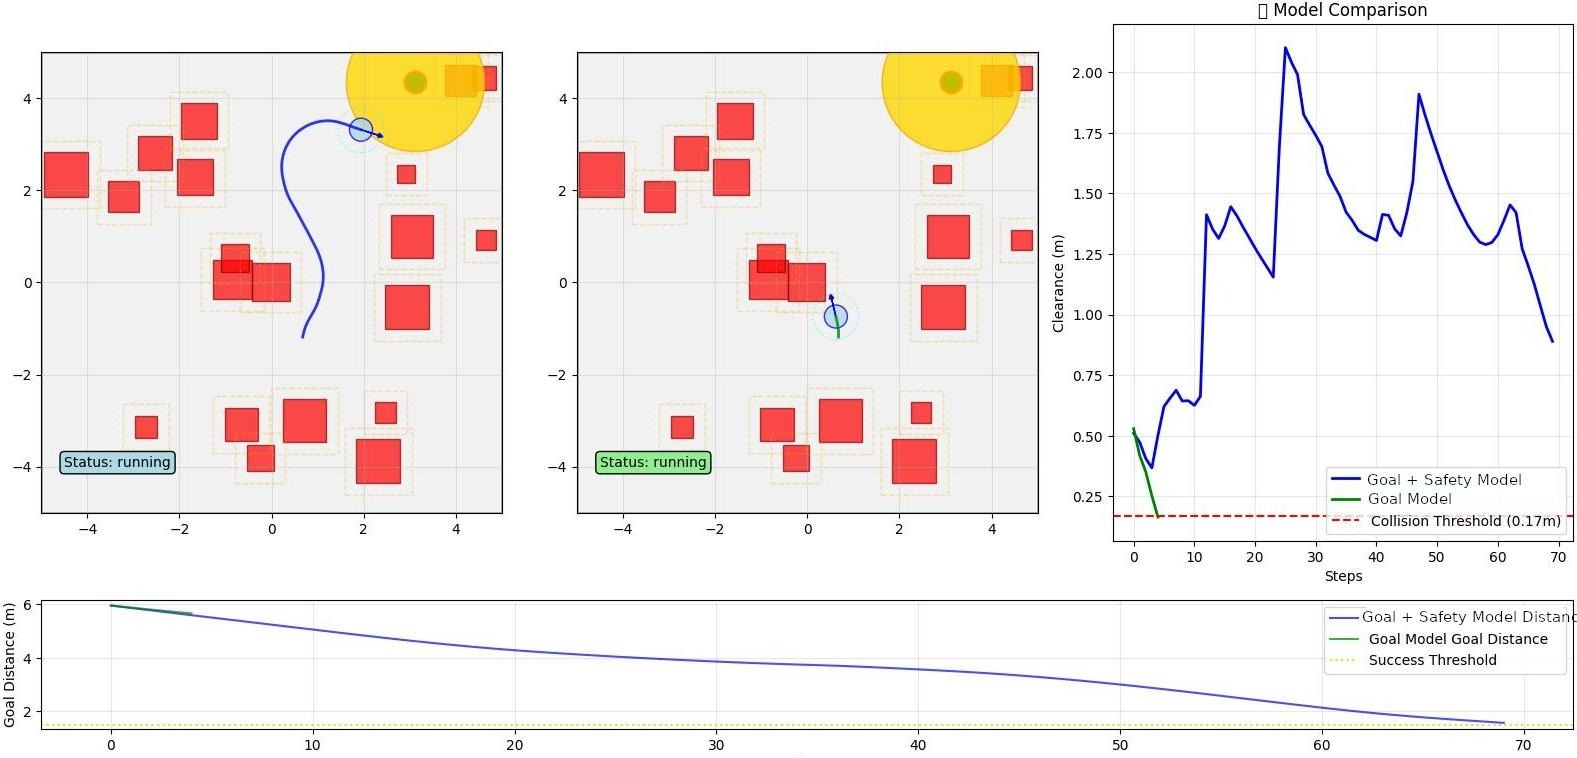
\includegraphics[width=\columnwidth]{safety_vs_goal_results.jpeg}
    \caption{Visual comparison of a safety-aware model vs. a goal-only model. The top-right plot shows that the safety-aware agent (blue) consistently maintains a higher clearance from obstacles than the goal-only agent (green), which quickly violates the collision threshold (red dashed line).}
    \label{fig:visual_comparison}
\end{figure}

\subsection{Observations and Analysis}
Our preliminary results validate our implementation and highlight the core trade-offs in safe navigation.
First, our training process is stable and effective. The TensorBoard logs for both the \textbf{Safety-Only} (Fig.~\ref{fig:safety_training}) and \textbf{Goal-Only} (Fig.~\ref{fig:goal_training}) models show steady convergence of losses and stabilization of rewards, confirming our implementation is working as expected.

Second, the models learn distinct, predictable behaviors. The Safety-Only agent produces qualitatively successful collision-avoidance maneuvers, as seen in the smooth trajectories of Fig.~\ref{fig:safety_only}. However, as the quantitative results in Table~\ref{tab:baseline_comparison} show, this focus on safety comes at the cost of task performance, with only a 50\% success rate. Conversely, the Goal-Only agent learns to pursue the goal but is demonstrably unsafe, colliding in 70\% of episodes. The direct comparison in Fig.~\ref{fig:visual_comparison} visualizes this perfectly: the safety-aware agent maintains clearance, while the goal-only agent's trajectory leads to a collision.

Finally, the \textbf{Balanced} model, which uses a naive reward-weighting scheme, fails to find a good compromise, yielding a high collision rate of 63.3\%. These results strongly motivate the need for the CAC architecture. The objective is to merge the robust safety of the "Safety-Only" policy with effective goal-seeking behavior—something simple reward mixing cannot achieve. This sets the stage for implementing the Stage 2 restricted policy update, which is designed to improve task performance while preserving the safety learned in Stage 1.

\section{Brief Summary of Reported Results \& Our Evaluation Plan}
\textbf{Reference Paper Results.} In the CartPole task, both the intermediate safe policy and the final policy remain within safety bounds, while the final policy successfully reaches the target position (Fig.\,3–4, p.\,4). In the underwater navigation task, CAC achieves significantly higher success rates ($\sim\!86\%$) and lower collision rates ($\sim\!11\%$) compared to baselines (Table~II, p.\,6). The paper also shows that the safety critic value correlates well with empirical safety metrics (Fig.\,5, p.\,5), which we will seek to reproduce \cite{Xie2025CAC}.

\textbf{Our Midterm Status.} We have accomplished the following: (i) finalized the problem definition and central reference; (ii) implemented the two-stage training architecture with a SAC backbone; (iii) developed a 2D navigation simulator with range-based sensing and random obstacle generation; (iv) unit-tested the CBF/CLF reward functions and the restricted-gradient projection; and (v) generated the comprehensive preliminary results shown above, which validate our implementation and motivate subsequent experiments.

\textbf{Planned Evaluation.} Our final report will compare the full CAC implementation against the three baselines presented in Table~\ref{tab:baseline_comparison}. We will measure success rate, collision rate, path length, and the correlation between the safety critic's value and the empirical safe-episode rate.

\section{Bottlenecks and Ultimate Challenges}
\textbf{Near-term Bottlenecks.}
\begin{itemize}
    \item \textbf{CBF and CLF Design:} Hand-designed functions may be brittle. While learning CBFs is a promising alternative, it raises new questions about verification and generalization \cite{Guerrier2024Survey,Harms2024NeuralCBF}.
    \item \textbf{Model Uncertainty:} CBF-based methods can be sensitive to mismatches between the simulated and real dynamics.
    \item \textbf{Safe Exploration:} Ensuring safety even during early training remains a challenge, often requiring careful reward shaping \cite{Ranjan2024BarrierShaping}.
    \item \textbf{Scalability:} Maintaining multiple critics for safety and task objectives increases computational overhead and may affect sample efficiency.
\end{itemize}

\textbf{Ultimate Challenges.}
\begin{itemize}
    \item \textbf{Formal Guarantees:} Extending critic values to certified, long-horizon safety guarantees under distribution shift is an open problem.
    \item \textbf{Partial Observability:} Using CBFs with raw sensor data (e.g., from LiDAR or cameras) without full state estimation is difficult \cite{Harms2024NeuralCBF}.
    \item \textbf{Sim-to-Real Transfer:} Unmodeled effects like disturbances, delays, and contacts challenge safety assumptions made in simulation.
    \item \textbf{Multi-Agent Systems:} Extending safety certificates to interactive human-robot or multi-robot scenarios is a major research frontier.
\end{itemize}

\section{Timeline \& Next Steps (Final Report Preview)}
\textbf{Week 1--2:} Finalize environments and hyperparameters; replicate CartPole safety results. \\
\textbf{Week 3--4:} Run full CAC experiments and ablations on 2D/AUV navigation benchmarks.\\
\textbf{Week 5:} Conduct stress tests (e.g., sensor noise, dynamics mismatch) and analyze critic calibration.\\
\textbf{Week 6:} Draft final report and presentation slides; prepare figures and results.

\section{Conclusion}
We have selected a safety-critical navigation application and are analyzing a recent hierarchical RL algorithm (CAC) that uses CBF-derived rewards to create an explicit \emph{safety critic}. Our midterm report establishes the problem, methodology, and a clear evaluation plan. Our final report will deliver a comprehensive experimental analysis, including ablations and a discussion on the practical feasibility of this approach for real-world robot deployment.

\section*{Acknowledgment}
A link to a short demonstration video will be included in our final submission.

\section*{Code Availability}
The code for our implementation and experiments is available at: \url{https://github.com/Jeevan-HM/RL-in-Robotics/tree/midterm}

\bibliographystyle{IEEEtran}
\begin{thebibliography}{99}

\bibitem{Xie2025CAC}
J.~Xie, S.~Zhao, L.~Hu, and H.~Gao, ``Certificated Actor--Critic: Hierarchical Reinforcement Learning with Control Barrier Functions for Safe Navigation,'' \emph{arXiv preprint arXiv:2501.17424}, 2025.

\bibitem{Guerrier2024Survey}
M.~Guerrier, H.~Fouad, and G.~Beltrame, ``Learning Control Barrier Functions and their Application in Reinforcement Learning: A Survey,'' \emph{arXiv:2404.16879}, 2024.

\bibitem{Ranjan2024BarrierShaping}
A.~Ranjan, S.~Agrawal, A.~Jain, P.~Jagtap, S.~Kolathaya, and N.~Nilaksh, ``Barrier Functions Inspired Reward Shaping for Reinforcement Learning,'' in \emph{Proc.\ IEEE ICRA}, 2024, pp.~1--7. (arXiv:2403.01410).

\bibitem{Kalaria2024DOB}
D.~Kalaria, Q.~Lin, and J.~M.~Dolan, ``Disturbance Observer-based Control Barrier Functions with Residual Model Learning for Safe Reinforcement Learning,'' \emph{arXiv:2410.06570}, 2024.

\bibitem{Harms2024NeuralCBF}
M.~Harms, M.~Kulkarni, N.~Khedekar, M.~Jacquet, and K.~Alexis, ``Neural Control Barrier Functions for Safe Navigation,'' \emph{arXiv:2407.19907}, 2024.

\end{thebibliography}

\end{document}